\chapter{The \textsc{Tavor Framework}}
\label{chapter:tavorFramework}

The main goal of \textsc{Tavor} is to provide functionality for the automatic generation, alteration and reduction of test data which conforms to a predefined structure. Programs oftentimes need to process complex data structures that allow for an enormous number of possible variants. Such programs are therefore hard to test, since a tester has to consider every important variant for testing purposes. To construct the input data manually is time-intensive and error-prone. \textsc{Tavor} can be used to automate the generation of this data, to alter existing data and to apply delta-debugging to systematically reduce existing data according to a predefined structure and its constraints.

\begin{figure}[hb]
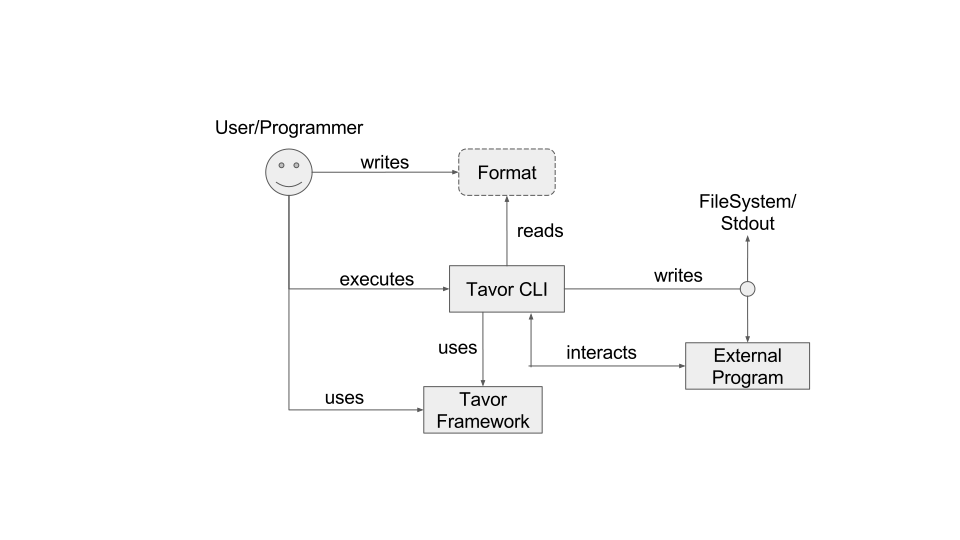
\includegraphics[width=0.8\textwidth]{images/tavor-interactions.pdf}
\caption{\textsc{Tavor}'s subsystems}
\label{fig:tavor-interactions}
\end{figure}

Figure~\ref{fig:tavor-interactions} depicts the interactions of the \textsc{Tavor} subsystems. In order to interact with an external program a user first needs to define a data model which describes the structure of the expected inputs to the program. The \textsc{Tavor framework} provides its own format to define such data models, which covers all functionality of the framework. Please refer to Chapter~\ref{chapter:tavorFormat} for a detailed description of the \textsc{Tavor format} and its capabilities. Next, the \textsc{Tavor CLI} can be used to interact with an external program. Interactions such as fuzzing or delta-debugging are also provided by the \textsc{Tavor CLI}, which is described in more detail in Chapter~\ref{chapter:tavorFormat}. The \textsc{Tavor CLI} relies heavily on the algorithms and data structures provided by the \textsc{Tavor framework}. The framework's design goals as well as its components and their interactions are the main focus of the subsequent sections of this chapter.

\section{Components}
\label{sec:components}

The \textsc{Tavor framework} offers various components which are depicted in Figure~\ref{fig:tavor-components}. There are three utility components, i.e., \texttt{Tokens}, \texttt{Parsers} and \texttt{Logging}, as well as three components offering access to different kinds of algorithms, i.e., \texttt{Fuzzing Strategies}, \texttt{Fuzzing Filters} and \texttt{Reducing Strategies}.

\begin{figure}[ht]
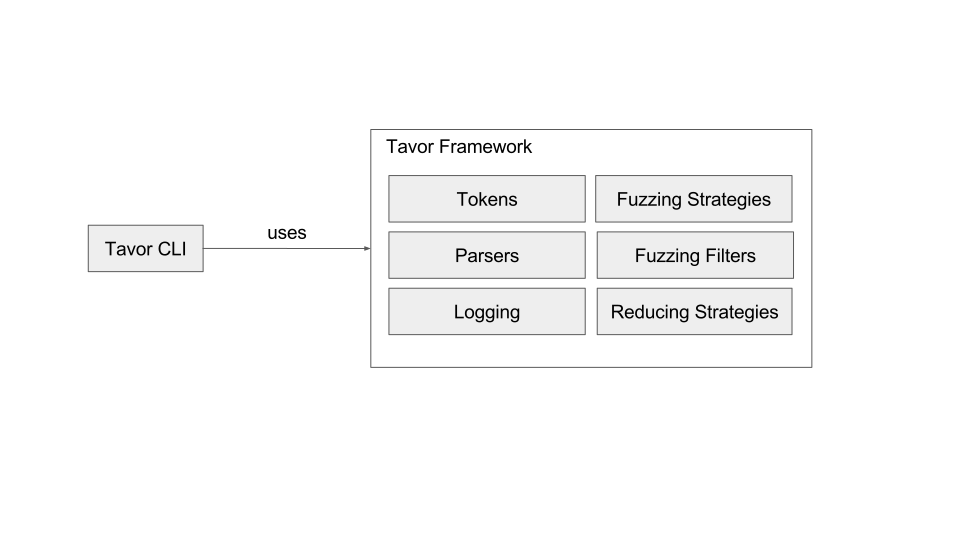
\includegraphics[width=1.0\textwidth]{images/tavor-components.pdf}
\caption{Components of the \textsc{Tavor framework}}
\label{fig:tavor-components}
\end{figure}

In order to combine both, fuzzing and delta-debugging, all implemented methods of the \textsc{Tavor framework} operate on one internal model-based structure. This structure is basically a graph of nodes that are called \texttt{token graphs} throughout the \textsc{Tavor framework}. Each node represents an instance of a \texttt{token} of a framework-defined type. A token graph can either be directly instantiated or by parsing a format file using the \texttt{Parsers} component of the \textsc{Tavor framework}. The \texttt{Logging} component provides extensive logging for debugging the handling of tokens. The granularity of logged output can be controlled by specifying the desired log level, i.e., the debug level reports the widest range of information while the error level only informs about occurred errors.

Instead of focusing on only one technique \textsc{Tavor}'s components have been kept generic. Dedicated techniques and heuristics can be implemented and executed independently. All of these components operate on tokens. In order to generate permutations of a specific token, i.e., unique arrangements of the token's values, \texttt{fuzzing strategies} are used. A token itself is not fixed to a static definition but can be changed by \texttt{fuzzing filters} to apply additional techniques such as boundary-value analysis of ranges. For delta-debugging so called \texttt{reducing strategies} can be implemented and used.

Every algorithm of the \textsc{Tavor framework} has to be deterministic, since determinism has the advantage that it eases debugging problems and enables the reproduction of results that are sent to external programs. Therefore, no functionality is allowed to have its own source or seed of randomness. Instead, a common interface that defines a random generator is used throughout the framework. An implementation of this interface has to be deterministic given the same seed of randomness. The decision of keeping code deterministic was also applied to concurrent code and tests, making it possible to reproduce the same output given the same random seed and version of the framework.

The following subsections present \textsc{Tavor}'s fundamental implementation decision as well as its main components \texttt{Tokens}, \texttt{Fuzzing Strategies}, \texttt{Fuzzing Filters} and \texttt{Reducing Strategies} in more detail.

\section{Tokens}
\label{sec:tokens}

The basic building blocks of the \textsc{Tavor framework} are its \emph{tokens}. These tokens differ from \emph{lexical analysis tokens} in the following way: They represent not just a group of characters, but different kinds of data with additional properties and abilities. Tokens can be constant integers and strings of all kind as well as dynamic data such as integer ranges, sequences and character classes. Furthermore, tokens can encapsulate other tokens to group them together and to create building blocks that can be reused to, for example, repeat a group of tokens. Tokens can have states, conditions and can perform operations such as arithmetic. They can create new tokens dynamically and can depend on other tokens to generate data. Tokens are basically the foundation of the framework and every algorithm for parsing, fuzzing and delta-debugging is relying on them.

A \emph{permutation} of a token is a specific arrangement of its values. Every token type has its own arrangement implementation and every token instance can have its own values. However, the set of permutations is unique for a specific token type and values, as is the order of these permutations. For example a token holding a range of numbers from \enquote{4} to \enquote{6} has 3 possible permutations: \enquote{4}, \enquote{5} and \enquote{6}. The first permutation of this token is \enquote{4} and the third permutation is \enquote{6}. Even though this demonstrates that a token can represent many permutations, every token can hold only one permutation at any given time. Therefore, every token implementation should differentiate between an internal and external representation. Since it is necessary to save the possible values internally but to forward the current value externally. This distinction is especially important for token types that generate new tokens out of their internal representation. The original internal tokens should not be connected to the external ones, since it would be otherwise possible to change the internal representation without any contract.

Many of the algorithms in the \textsc{Tavor framework} build upon the assumption that the processed token graphs are acyclic. This decision allows for easier implementations and usage since no guards and functionality have to implemented to deal with infinitely running algorithms and unwanted repetitions. Hence, while the internal structure allows tokens to have loops in their graphs, each loop must be unrolled before it can be used with the algorithms of the \textsc{Tavor framework}, i.e., the bodies of repetitions are copied N-times instead of the original repetition. An example for a token graph with a loop is given in Figure~\ref{fig:unroll-loop} which is then unrolled twice resulting in the graph of Figure~\ref{fig:unroll-unrolled}.

\begin{figure}[ht]
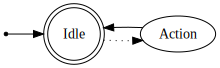
\includegraphics[height=0.125\textwidth]{images/unroll-loop.pdf}
\caption{Example for a Graph with a Loop}
\label{fig:unroll-loop}
\end{figure}

\begin{figure}[ht]
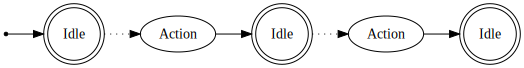
\includegraphics[height=0.1\textwidth]{images/unroll-unrolled.pdf}
\caption{Example for an Unrolled Graph}
\label{fig:unroll-unrolled}
\end{figure}

Every token implements at least the basic \emph{Token Interface}, which specifies methods for generating, replicating, permutating and parsing. Additional token interfaces add specific functionality to a token. The \emph{List Interface}, for example, states that a token can have child tokens and specifies methods to access them.

The Token Interface is the base interface of all tokens. Its operations can be grouped into the following categories:

\begin{itemize}
\item \textit{Generation} to output the external representation of the token.
\item \textit{Replication} to create an exact copy of the token.
\item \textit{Permutation} to permutate the token.
\item \textit{Parsing} to parse arbitrary input to permutate the token.
\end{itemize}

Subsection~\ref{subsec:tokens-smiley} presents an example token implementation which exemplifies the above-mentioned fundamental token concepts. Subsequently Subsection~\ref{subsec:tokens-advanced-concepts} elaborates on advanced token concepts, which are for instance necessary to model repetitions or constraints.

\subsection{Example Implementation - The \textsc{Smiley} Token}
\label{subsec:tokens-smiley}

This subsection illustrates the implementation of a basic \textsc{Tavor} Token, thus explaining the fundamental token operations by example. Since the \textsc{Tavor framework} is written in the programming language \textsc{Go}, the following implementations are written in \textsc{Go} as well. \textsc{Go} is an open source programming language created at Google. The language is garbage collected which allows the following examples to be nearly uncluttered of memory handling. Furthermore, \textsc{Go}'s C-like syntax should be widely readable with the exceptions of three operators: The \emph{short variable declaration} operator \enquote{:=} declares and initializes a variable using the value and variable type of the right-hand side of the operator. The range operator allows the programmer to iterate over an array using a for-loop, e.g., \texttt{for i, p := range people} iterates over the variable \texttt{people} with \texttt{i} holding the index and \texttt{p} holding the item of the current iteration. Lastly, the \enquote{go} operator starts the encapsulated function call in a new coroutine.

Consider a token defining a smiley which has eyes, a mouth and can have a nose. The token should be able to generate different permutations of smilies and even parse them. This example uses two different kinds of eyes: \enquote{\texttt{:}} and \enquote{\texttt{;}}, an optional nose \enquote{\texttt{-}} and three different kinds of mouths: \enquote{\texttt{)}}, \enquote{\texttt{(}} and \enquote{\texttt{D}}. Thus, we allow for instance the smiley \enquote{\texttt{;-D}}, but not \enquote{\texttt{:-<}}. This example should in general show how easy it is to create new token types. It must be noted that this example could be easily implemented with the available token types or with the \textsc{Tavor format} shown in Listing~\ref{lst:smiley-format}.

\begin{listing}
\caption{Smiley \textsc{Tavor format}}
\label{lst:smiley-format}
\begin{gocode}
START = [:;] ?("-") [)(D]
\end{gocode}
\end{listing}

Listing~\ref{lst:smiley-data-structure} shows the basic data structure of the \textsc{Smiley} Token. Since the \textsc{Smiley} Token has to hold three different types of information, it is necessary to create a structure. Instead of directly using the characters for the eyes and mouth in the structure, only indices are used. This is not necessary but helps to separate the constant data from the permutation of the token. Using this data structure the smiley \enquote{\texttt{;-D}} would be represented with the composite literal \texttt{Smiley\string{eyes:~1, nose:~true, mouth:~2\string}}. The structure must implement the Token Interface, which is grouped into method categories as described in Section~\ref{sec:tokens}. The implementations of these categories are now presented in the remainder of this section.

\begin{listing}
\caption{Smiley Data Structure}
\label{lst:smiley-data-structure}
\begin{gocode}
var (
	eyes   = ":;"
	mouths = ")(D"
)

type Smiley struct {
	eyes  int
	nose  bool
	mouth int
}
\end{gocode}
\end{listing}

The \textit{Generation} category of the Token Interface deals with the output of the current permutation. To implement this category at least the \texttt{String} method has to be implemented, which returns the textual representation of the token's current permutation. The \texttt{String} method for the \textsc{Smiley} Token is shown in Listing~\ref{lst:smiley-string-method}, and returns for the smiley \texttt{Smiley\string{eyes:~1, nose:~true, mouth:~2\string}} the string \enquote{\texttt{;-D}}. Since the internal representation should not be accessible by the token's user, no safeguards, e.g., for accessing array items by their indices, are necessary.

\begin{listing}
\caption{Smiley \texttt{String} Method}
\label{lst:smiley-string-method}
\begin{gocode}
func (s *Smiley) String() string {
	nose := ""
	if s.nose {
		nose = "-"
	}

	return string(eyes[s.eyes]) + nose + string(mouths[s.mouth])
}
\end{gocode}
\end{listing}

The \textit{Replication} category deals with replicating tokens, i.e., with creating copies of tokens. The \texttt{Clone} method is the only replication function required by the Token Interface. Note that the new token must be independent of the original token, i.e., that each \texttt{Clone} function needs to perform a deep rather than a shallow copy of its data. For the \textsc{Go} programming language this means that token internal slices, maps, structures and token children must be copied as well. The implementation of the \texttt{Clone} method for the \textsc{Smiley} Token is shown in Listing~\ref{lst:smiley-clone-method}.

\begin{listing}
\caption{Smiley \texttt{Clone} Method}
\label{lst:smiley-clone-method}
\begin{gocode}
func (s *Smiley) Clone() token.Token {
	return &Smiley{
		eyes:  s.eyes,
		nose:  s.nose,
		mouth: s.mouth,
	}
}
\end{gocode}
\end{listing}

The \textit{Permutation} category handles the set of permutations for a token as well as its current permutation. The method \texttt{Permutations} defines how many permutations a single token holds. The \textsc{Smiley} Token has a constant number of 12 permutations, since the amount of eyes, mouths and noses is constant. Other tokens such as ranges of integers depend on their configuration. The implementation of the \texttt{Permutations} method for the \textsc{Smiley} Token is shown in Listing~\ref{lst:smiley-permutations-method}.

\begin{listing}
\caption{Smiley \texttt{Permutations} Method}
\label{lst:smiley-permutations-method}
\begin{gocode}
func (s *Smiley) Permutations() uint {
	return uint(len(eyes) * 2 * len(mouths))
}
\end{gocode}
\end{listing}

The method \texttt{PermutationsAll} returns the number of permutations of the token itself and all its children. Since the \textsc{Smiley} Token has no children, it is the same as \texttt{Permutations} which is shown in Listing~\ref{lst:smiley-permutationsAll-method}. However, it is important to note that calculating the amount of permutations is not always a straightforward task. Consider for instance the \emph{Concatenation Token} representing a sequence of tokens, which requires all of its children to be present, and the \emph{One Token}, which requires exactly one of its children to be present. These two tokens have very different permutation calculations. For the Concatenation Token the product of its children's \texttt{PermutationsAll} result is calculated using $\prod_{i=1}^{token. NumChildren} Token.Child(i).PermutationsAll()$ while for the One Token the sum of its children's \texttt{PermutationsAll} result is calculated using $\sum_{i=1}^{token. NumChildren} Token.Child(i).PermutationsAll()$.

\begin{listing}
\caption{Smiley \texttt{PermutationsAll} Method}
\label{lst:smiley-permutationsAll-method}
\begin{gocode}
func (s *Smiley) PermutationsAll() uint {
	return s.Permutations()
}
\end{gocode}
\end{listing}

The \texttt{Permutation} method completes the \textit{Permutation} category. It sets a distinct permutation of the token, i.e., calling the method with the integer 11 results in \texttt{Smiley\string{eyes:~1, nose:~true, mouth:~2\string}} which represents the \texttt{;-D} smiley. The implementation of the \texttt{Permutation} method for the \textsc{Smiley} Token is shown in Listing~\ref{lst:smiley-permutation-method}, and has been intentionally been made inefficiently to keep the example simple.

\begin{listing}
\caption{Smiley \texttt{Permutation} Method}
\label{lst:smiley-permutation-method}
\begin{gocode}
func (s *Smiley) Permutation(i uint) error {
	if i < 0 || i >= s.Permutations() {
		return NewPermutationErrorIndexOutOfBound()
	}

	p := uint(0)
	for eyes := range eyes {
		for _, nose := range []bool{false, true} {
			for mouth := range mouths {
				if i == p {
					s.eyes = eyes
					s.nose = nose
					s.mouth = mouth

					return nil
				}

				p++
			}
		}
	}

	return nil
}
\end{gocode}
\end{listing}

Finally, the \texttt{Parsing} category, which is the last category of the Token Interface, deals with parsing the token from an input. Listing~\ref{lst:smiley-parse-method} shows the \texttt{Parse} method of the \textsc{Smiley} Token. The implementation may look very verbose, but it is necessary to handle every syntax error to generate adequate parsing errors. Note that these messages could be further improved by not only stating that something was expected, but actually giving examples on what has been expected.

\begin{listing}
\caption{Smiley \texttt{Parse} Method}
\label{lst:smiley-parse-method}
\begin{gocode}
func (s *Smiley) Parse(parser InternalParser, cur int) (int, []error) {
	if cur+2 > parser.DataLen {
		return cur, []error{errors.New("Out of data for a smiley")}
	}

	if i := strings.IndexRune(eyes, parser.Data[cur]); i != -1 {
		s.eyes = i
	} else {
		return cur, []error{errors.New("Expected some eyes")}
	}
	cur++

	if parser.Data[cur] == '-' {
		s.nose = true
		cur++
	} else {
		s.nose = false
	}
	if cur >= parser.DataLen {
		return cur, []error{errors.New("Out of data for a mouth")}
	}

	if i := strings.IndexRune(mouths, parser.Data[cur]); i != -1 {
		s.mouth = i
	} else {
		return cur, []error{errors.New("Expected a mouth")}
	}
	cur++

	return cur, nil
}
\end{gocode}
\end{listing}

The \textsc{Smiley} Token can then be used to create structures like with any other token of the framework. However, to give an easier example, it will be used alone. Listing~\ref{lst:working-with-smiley} creates a new \textsc{Smiley} Token, permutates over all permutations and parses a string. Each step is printed to STDOUT. Resulting in the output shown in Listing~\ref{lst:working-with-smiley-output}.

Please note, that the smiley token has been used to demonstrate, which standard methods each token type needs to implement. Of course, the \textsc{Tavor framework} already offers a wide range of token types allowing to represent arbitrary formats. Chapter~\ref{chapter:tavorFormat} gives an overview of the format options that are already implemented by the tokens of the \textsc{Tavor framework}.

\begin{listing}
\caption{Working with the \textsc{Smiley} Token}
\label{lst:working-with-smiley}
\begin{gocode}
func main() {
	s := Smiley{}

	fmt.Print("Permutations:")
	for i := uint(0); i < s.Permutations(); i++ {
		s.Permutation(i)
		fmt.Print(" ", s.String())
	}
	fmt.Println()

	p := NewInternalParser(":-D")
	_, errs := s.Parse(p, 0)
	if errs != nil {
		panic(errs)
	}

	fmt.Println("Parsed:", s.String())
}
\end{gocode}
\end{listing}

\begin{listing}
\caption{Output of Smiley Example}
\label{lst:working-with-smiley-output}
\begin{textcode}
Permutations: :) :( :D :-) :-( :-D ;) ;( ;D ;-) ;-( ;-D
Parsed: :-D
\end{textcode}
\end{listing}

\subsection{Advanced Token Concepts}
\label{subsec:tokens-advanced-concepts}

While \textsc{Tavor} actually lacks the \textsc{Smiley} Token introduced in Subsection~\ref{subsec:tokens-smiley}, it offers a wide range of different token types, which can be used to model arbitrary formats.
The following categories of tokens give an excerpt of the different tokens supported by \textsc{Tavor}:

\begin{itemize}
\item \textit{Primitive} Tokens do not reference other tokens, i.e., they are vertices in the token graph without any outgoing edges. These tokens solely implement the basic Token Interface. The plainest types are the \texttt{Integer} and \texttt{String} Tokens, which represent constant data of numbers and texts, e.g., \enquote{1234} and \enquote{"Hello World}. Other examples of this category, such as the as \texttt{RangeInt} which allows to define a range of integers, are dynamic, i.e., can have more than one permutation, but can represent only one permutation at any given time. Another example is the \texttt{CharacterClass} Token, most commonly known from regular expressions, which allows to define character class definitions such as \texttt{[ACE]} allowing either one of the characters \enquote{A}, \enquote{C} or \enquote{E}.
\item \textit{List} Tokens contain a list of child tokens. Additionally to the basic Token Interface these tokens also implement the List Interface, which provides methods to operate on the token's children. At the moment of writing the token types \texttt{Concatenation}, \texttt{Once}, \texttt{One} and \texttt{Repeat} are currently supported. The \texttt{Concatenation} (resp. \texttt{Once}) Token requires all children to be present in the defined order (resp. an arbitrary order). The \texttt{One} Token allows to define lists were exactly one child token is present in every permutation. Finally the \texttt{Repeat} Token is used to repeat defined tokens for a specified amount of times.
\item \textit{Constraint} Tokens are used to bind tokens to constraints, e.g., the \texttt{Optional} Token expresses that the wrapped token may or may not be present.
\item \textit{Expression} Tokens are used to define formulas, consisting of one or more token, which can be resolved to a single value, which is again a token. Such tokens can be for example arithmetically such as \texttt{ArithmeticAdd}, \texttt{ArithmeticSub}, \texttt{ArithmeticMul} and \texttt{ArithmeticDiv} which allow simple calculations of numbers. The \texttt{BooleanTrue} and \texttt{BooleanEqual} are another example of expression tokens, which belong to the scope of boolean algebra.
\item \textit{Statement} Tokens are used to handle control flows in token graphs, e.g., the \texttt{If} Token uses a boolean expression to guard a child token which is only active if the expression is true.
\item \textit{Variable} Tokens have been implemented in order to be able to reuse and interact with generated values at another place in a token graph.
\end{itemize}

Every token type and interface can have its own \textit{token attributes}, which are used to access meta information about a token. Each List token, for instance, provides the attributes \texttt{Count} to retrieve to the number of its child tokens, \texttt{Item(i)} to refer to its i-th child and \texttt{Unique} to refer to an arbitrary but unique child of the list.

Consider Figure~\ref{fig:automaton-simple-format}, it shows an automaton which allows an \enquote{a} character, followed by two to four \enquote{b}, an optional \enquote{c} and a concluding \enquote{d}. The token graph representing this format is shown in Figure~\ref{fig:token-graph-simple-format}. It is rooted in a \texttt{Concatenation} Token which has four child tokens. The starting and concluding tokens are simply constant strings, i.e., they need to be present in every permutation. The repetition of \enquote{b} is expressed using a \texttt{Repeat} Token with the configuration \texttt{from=2} and \texttt{to=4}. In order to model that the String Token \enquote{b} is optional it is wrapped in an \texttt{Optional} Token.

\begin{figure}
\begin{center}
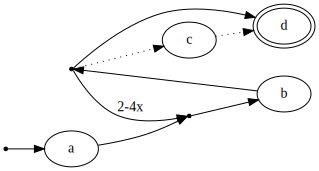
\includegraphics[height=0.3\textwidth]{images/tavor-simple-format.pdf}
\caption{Automaton of Simple Format Definition}
\label{fig:automaton-simple-format}
\end{center}
\end{figure}

\begin{figure}[ht]
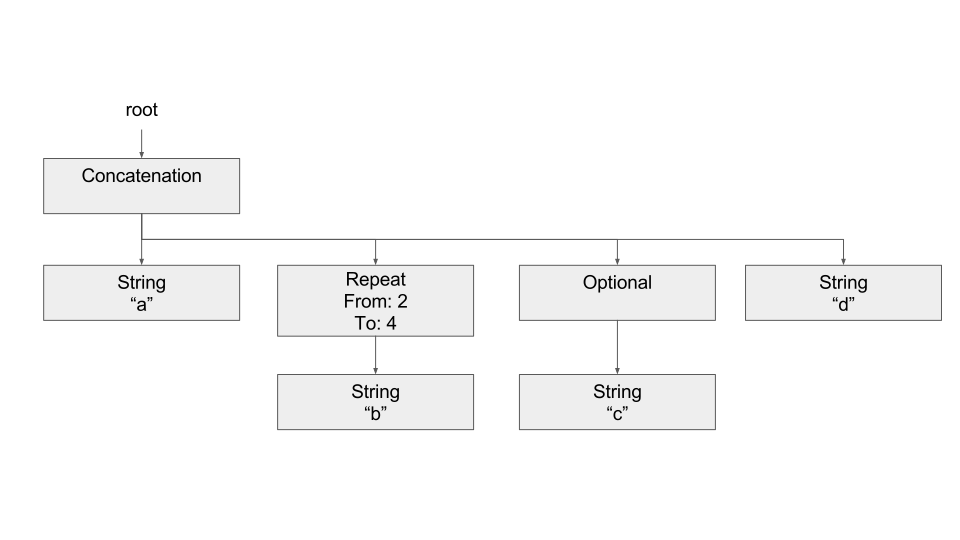
\includegraphics[width=1.0\textwidth]{images/tavor-simple-format-token-graph.pdf}
\caption{Token Graph of Simple Format Definition}
\label{fig:token-graph-simple-format}
\end{figure}

Most algorithms of the \textsc{Tavor framework} traverse a token graph and perform a certain operation on each traversed token. Auxiliary functions are provided by the framework to fulfill this purpose. One of these functions is \texttt{Walk} which is depicted as pseudo code in Listing~\ref{lst:walk-func}. It receives two input parameter: the \texttt{root} Token which needs to be traversed and the function \texttt{walkFunc} which is called for each traversed token. A queue is used to systematically traverse the token graph. Remember, no cycles are allowed within a token graph. Hence, no loop-detection needs to be implemented. Tokens that implement the Forward Interface, which reference a single token, are handled in Line~14, which pushes the referenced child for later processing onto the queue. The List Interface is implemented by those token types who refer to a list of child tokens, hence the loop from Lines~16-18 is used to add all referenced children onto the queue.

\begin{listing}
\caption{Token Graph Walk Function}
\label{lst:walk-func}
\begin{gocode}
func Walk(root Token, walkFunc func(token Token) error) error {
	queue := NewQueue()
	queue.Push(root)

	for !queue.Empty() {
		token := queue.Pop()

		if err := walkFunc(token); err != nil {
			return err
		}

		switch t := token.(type) {
		case Forward:
			queue.Push(t.Get())
		case List:
			for i := t.Len() - 1; i >= 0; i-- {
				queue.Push(t.Get(i))
			}
		}
	}

	return nil
}
\end{gocode}
\end{listing}

\section{Fuzzing Strategies}
\label{sec:fuzzingStrategies}

The \textsc{Tavor framework} provides the concept of fuzzing strategies to generate permutations of a token graph according to a specific algorithm. There are two fundamental ways of token fuzzing. One is to deterministically choose one possible permutation, the other is to choose randomly out of all permutations of a token. All fuzzing strategies need to implement the following interface:

\begin{center} \texttt{type Strategy func(root Token, r rand.Rand) (chan bool, error)} \end{center}

This interface defines a single function, which initializes the strategy and then starts the first fuzzing iteration in a new coroutine. If an error is encountered during the initialization of the strategy, the error return argument is not nil. On success a channel is returned, which controls the fuzzing process. In the \textsc{Go} programming language channels are used to communicate among coroutines. For each completed iteration of the fuzzing strategy a value is returned by the channel. The caller of the strategy needs to put back a value into the channel, to initiate the calculation of the next fuzzing iteration. This passing of values is needed to avoid data races within the token graph. Note that the channel must be closed either when there are no more iterations, or in case the caller of the strategy wants to end the fuzzing process.

The \textsc{Tavor framework} provides the following default fuzzing strategies:
\begin{itemize}
\item The \emph{Random} strategy generates exactly one permutation of the passed in token graph by permuting each reachable token randomly. The determinism is dependent on the random generator and is therefore deterministic if the same random seed is used for initializing the random generator.
\item The \emph{AllPermutations} strategy deterministically generates all available permutations of a token.
\item The \emph{AllmostAllPermutations} strategy generates a subset of all available permutations by not covering all possible permutations of Repeat Tokens. This capability is especially helpful when less permutations are needed than provided by the \emph{AllPermutations} strategy.
\item The \emph{PermuteOptionals} strategy searches the graph for tokens implementing the \texttt{Optional Interface} and permutates over them by deactivating or activating them. The permutations always start from the deactivated states in order to generate minimum data first.
\end{itemize}

In order to provide a better understanding of the concept of fuzzing strategies we walk through an example implementation of a fairly basic fuzzing strategy in Section~\ref{sec:basic-fuzz-strategy}. Additionally, we offer in Section~\ref{sec:all-perm-fuzz-strategy} the pseudo code of the AllPermutations strategy, which is provided by the \textsc{Tavor framework}, and illustrate the algorithm using a walk-through for an example token graph.

\subsection{Basic Example Fuzzing Strategy}
\label{sec:basic-fuzz-strategy}

Consider a fuzzing strategy, which traverses the token graph looking for Integer tokens. Each integer having a value between 1 and 10 is incremented by one therefore replacing the original value. This strategy falls in the category of mutation-based fuzzing, since it does change the original model. It is also stateless since there is no need to keep track of current events between iterations. The graph is simply traversed and changed once per fuzzing iteration.

Listing~\ref{lst:sample-fuzz-strategy} depicts the pseudo code of the sample fuzzing strategy. First the channel to steer the fuzzing strategy is created in Line~2. Next a coroutine is started, see Lines~4-28, which makes use of the auxiliary function \texttt{Walk} to traverse the token graph. For each traversed token the function defined in Lines~8-19 is called, which is responsible to adapt the content of the currently traversed token. In case it is a Integer token holding a value between 1 and 10 the current token is adapted. After the traversal of the token graph the completion of the current iteration is reported to the \texttt{continueFuzzing} channel if at least one token has been adapted. Otherwise the channel is closed and the coroutine terminates.

\begin{listing}[ht]
\caption{Sample fuzzing strategy}
\label{lst:sample-fuzz-strategy}
\begin{gocode}
func NewSampleStrategy(root Token, r rand.Rand) (chan bool, error){
	continueFuzzing := make(chan bool)

	go func() {
		for {
			found := false

			err := Walk(root, func(token Token) error {
				intToken, ok := token.(*Integer)
				if !ok { return nil }

				v := intToken.Value()
				if v >= 1 && v <= 10 {
					found = true
					intTok.SetValue(v++)
				}

				return nil
			})
			if err != nil { panic(err) }
			if !found { break }

			continueFuzzing <- true
			if _, ok := <-continueFuzzing; !ok { return }
		}

		close(continueFuzzing)
	}()

	return continueFuzzing, nil
}
\end{gocode}
\end{listing}


One way to execute this strategy is by using the pseudo code shown in Listing~\ref{lst:call-example-fuzz-strat}. Note that the implemented strategy does not need a random generator, hence, this argument for the function can be \texttt{nil}. The produced output of this program is shown in Listing~\ref{lst:output-example-fuzz}, showing that the initial permutation \texttt{7 9} is fuzzed four times untill all constant integers have reached the value 11.

\begin{listing}
\caption{Callee of Example Fuzzing Strategy}
\label{lst:call-example-fuzz-strat}
\begin{gocode}
func main() {
	var root token.Token = lists.NewConcatenation(
		NewInteger(7),
		NewString(" "),
		NewInteger(9),
	)

	continueFuzzing, err := NewSampleStrategy(root, nil)
	if err != nil { panic(err) }

	for i := range continueFuzzing {
		fmt.Println(root.String())
		continueFuzzing <- i
	}
}
\end{gocode}
\end{listing}

\begin{listing}
\caption{Command Line Output of Example Fuzzing Strategy}
\label{lst:output-example-fuzz}
\begin{gocode}
8 10
9 11
10 11
11 11
\end{gocode}
\end{listing}

The last step when creating a fuzzing strategy is to make the strategy known to the \textsc{Tavor framework}. In order to do so, a register function is provided, which allows to register fuzzing strategies based on an identifier. This is especially needed for the Tavor CLI, which can execute a specific fuzzing strategy defined by a command line argument. The sample fuzzing strategy can be registered with the \textsc{Tavor framework} using the code shown in Listing~\ref{lst:register-sample-fuzz}.

\begin{listing}
\caption{Registering the sample fuzzing strategy}
\label{lst:register-sample-fuzz}
\begin{gocode}
func init() {
	strategy.Register("SampleStrategy", NewSampleStrategy)
}
\end{gocode}
\end{listing}

\subsection{The AllPermutations fuzzing strategy}
\label{sec:all-perm-fuzz-strategy}

The \emph{AllPermutations} fuzzing strategy is used to generate all permutations of a token graph in a deterministic manner. Consider the token graph in Figure~\ref{fig:all-perm-token-graph}, which describes a format allowing one or two \enquote{a} characters followed by \enquote{b}, \enquote{c} or \enquote{d} and concluded by an Optional Token \enquote{e}. Every token can tell how many permutations it has, i.e., the Concatenation Token has just one permutation as it always requires each of its children to be present. The Optional Token on the other hand is capable of two permutations, i.e., either its child token \enquote{e} is active or inactive.

In order to provide a better understanding on how the AllPermutations strategy operates, we first take a look at the computation of the number of possible permutations of the token graph. Consider Table~\ref{table:compute-All-perms}, it lists the formulas for calculating the number of possible permutations per token type. Applying these formulas to the token graph shown in Figure~\ref{fig:all-perm-token-graph}, results in $(1^1+1^2)*(1+(1+1))*(1+1) = 2 * 3 * 2 = 12$. These 12 supported permutations are listed in Listing~\ref{lst:permutations-allperm-token-graph}.

\begin{figure}
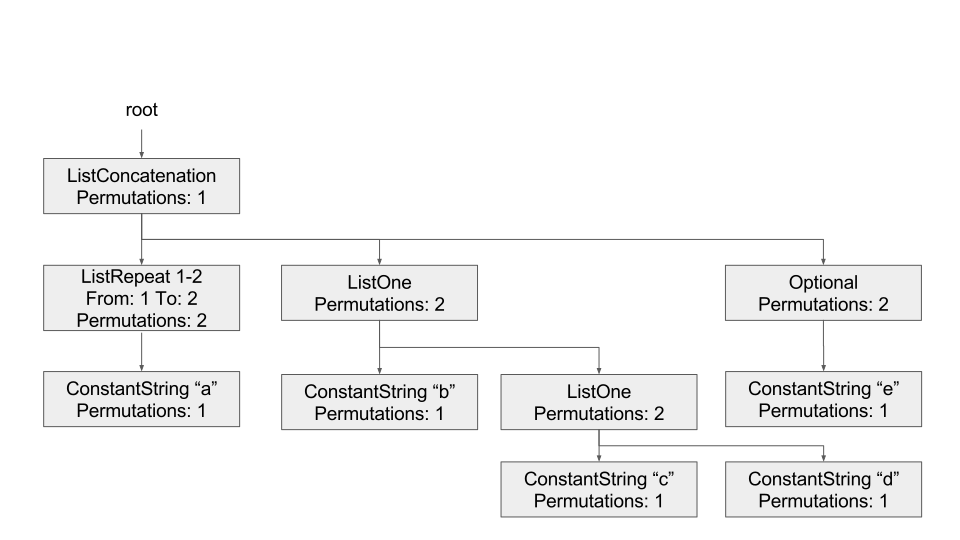
\includegraphics[width=1.0\textwidth]{images/tavor-all-permutation-token-graph.pdf}
\caption{AllPermutations example token graph}
\label{fig:all-perm-token-graph}
\end{figure}

\begin{table}[bt]
\caption{Computing PermutationsAll for different token types}
\label{table:compute-All-perms}
\center
\begin{tabular}{| l | l |}
\hline
  \textbf{Token Type}
& \textbf{Formula}
\tabularnewline
\hline
  Concatenation
& $\prod_{i=1}^{token.NumChildren} Token.Child(i).PermutationsAll()$
\tabularnewline
\hline
  Repeat
& $\sum_{i=From}^{To} Token.Child().PermutationsAll()^i$
\tabularnewline
\hline
  One
& $\sum_{i=0}^{token.NumChildren} Token.Child(i).PermutationsAll()$
\tabularnewline
\hline
  Optional
& $1 + token.Child().PermutationsAll()$
\tabularnewline
\hline
  String
& $1$
\tabularnewline
\hline
\end{tabular}
\end{table}

\begin{listing}
\caption{Permutation of AllPermutations example token graph}
\label{lst:permutations-allperm-token-graph}
\begin{gocode}
ab
aab
ac
aac
ad
aad
abe
aabe
ace
aace
ade
aade
\end{gocode}
\end{listing}

To iterate over all permutations of a token graph we view each token as a single digit in its own numeral system. In common numeral systems every digit has a fixed range. For instance, the decimal numeral system allows digits from 0 to 9. When incrementing a number over its range in one of those systems, a digit propagates an overflow to its neighboring higher digit and resets itself to the first digit of its range. Figure~\ref{fig:inc-decade-system} illustrates this propagation in the decimal numeral system on the calculations $0+1=1$, where no propagation takes place, $9+1=10$, where one digit propagates and $99+1=100$, where two digits propagate their overflow. A very similar concept is applied on token graphs when iterating over their permutations. In contrast to common number systems, each token may have a different range of values, i.e., an Optional Token can have the values $0$ and $1$ while a Repeat Token from 0 to 10 may have values from $0$ to $10$. In common numeral systems each digit has at most two neighboring digits, in comparison each token in a token graph may have a parent, siblings as well as child tokens which all need to be considered when calculating the next permutation.

\begin{figure}
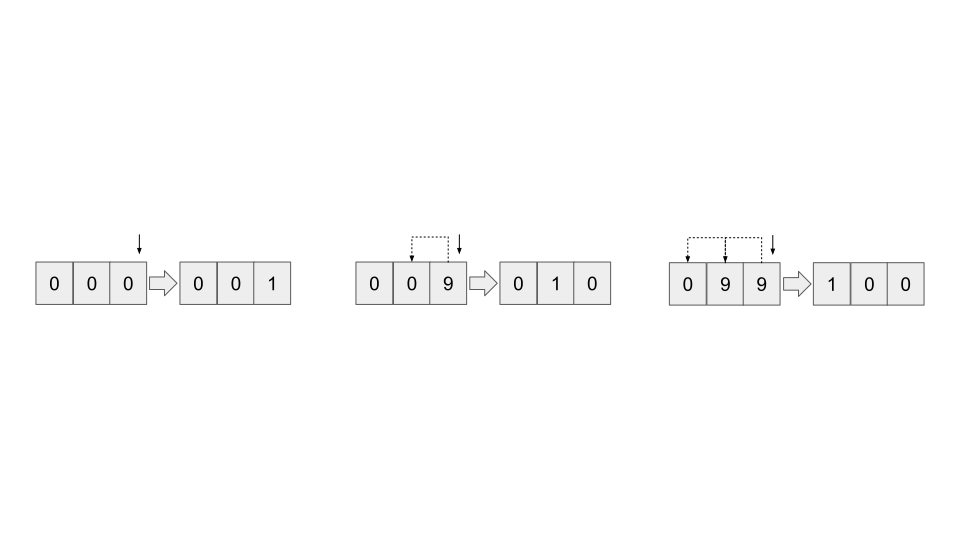
\includegraphics[width=1.0\textwidth]{images/tavor-increment-decade-system.pdf}
\caption{Incrementing in the decimal numeral system}
\label{fig:inc-decade-system}
\end{figure}

For calculating the next fuzzing iteration, i.e., the next permutation of the token graph, the AllPermutations strategy applies the following procedure on each token:
\begin{itemize}
\item If a token has children, first try to increment the permutation of its children. In case no overflow takes place, the next permutation has been successfully calculated.
\item If there are no children, or incrementing their current permutation results in an overflow, try to increment the current token's permutation. In case no overflow takes place, the next permutation has been successfully calculated.
\item If incrementing the permutation of the current token results in an overflow, propagate this overflow either to the neighboring higher sibling, or in case there are no siblings, the parent token. If the current token is the root token, this means the last permutation has been reached.
\end{itemize}

Figure~\ref{fig:all-perm-example} depicts the individual steps of the AllPermutations fuzzing strategy for the token graph shown in Figure~\ref{fig:all-perm-token-graph}. The solid arrows symbolize an increment instruction for a token, and the dashed arrows are used to depict the propagation of an overflow. The token graph is initialized with value 0 for all of its tokens, which represents the permutation \enquote{ab}. In order to step to the next permutation first an increment command is sent to the root token in iteration 0, which propagates this increment to its first child token the Repeat Token, which in turn also propagates to its child the String Token \enquote{a}. A String Token has only one permutation, hence, the increment command overflows setting the Repeat Token to value $1$, resulting in the permutation \enquote{aab}. In iteration 1 the same computation takes place, except that this time also the Repeat Token overflows setting the first One token to value $1$, resulting in permutation \enquote{ac}. This process continues until iteration 11, where the root token itself reports an overflow, hence no more permutations are available.

\begin{figure}[ht]
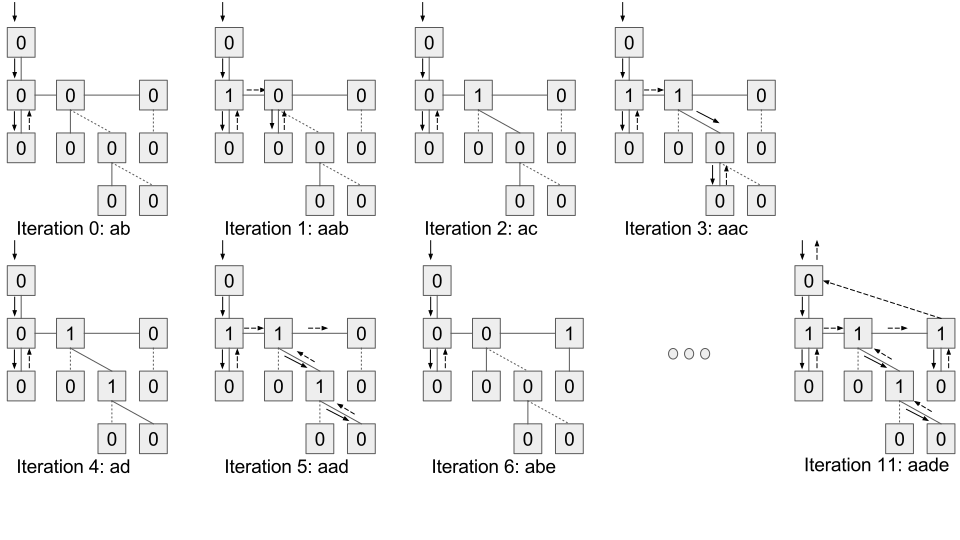
\includegraphics[width=1.0\textwidth]{images/tavor-all-permutations-example.pdf}
\caption{AllPermutations Iterations}
\label{fig:all-perm-example}
\end{figure}

Please refer to Appendix~\ref{chapter:AppendixTavorFramework} Listing~\ref{lst:pseudo-code-all-perm-strat} and Listing~\ref{lst:pseudo-code-all-perm-strat-helper} for the pseudo code of the AllPermutations fuzzing strategy.

\section{Fuzzing Filters}
\label{sec:fuzzingFilters}

In order to mutate a token graph, i.e., apply mutation-based fuzzing, the \textsc{Tavor framework} offers \emph{fuzzing filters}. Fuzzing filters do not change a specific permutation, but alter all permutations that may be generated with a specific token graph. All fuzzing filters need to implement the following interface:

\begin{center} \texttt{type Filter func(token Token) (Token, error)} \end{center}

This interface specifies a generic function, which applies the given filter onto a single token that is passed to the function. Therefore, the function's concern is only one token at a time. If an error is encountered during the filter execution, the error return argument is uninitialized. On success a replacement for the token is returned. If this replacement is not \texttt{nil}, it will replace the original token. Consider, for instance, a very basic filter that replaces each occurrence of the string \enquote{old} with the new constant string \enquote{new}. A possible implementation of this filter is shown in Listing~\ref{lst:tavor-example-filter}.

\begin{listing}[ht]
\caption{Sample Filter}
\label{lst:tavor-example-filter}
\begin{gocode}
func NewSampleFilter(token Token) (Token, error) {
	c, ok := token.(*String)
	if !ok || c.String() != "old" {
		return nil, nil
	}

	return NewString("new"), nil
}
\end{gocode}
\end{listing}

The \textsc{Tavor framework} offers a register function for fuzzing filters, which works along the same lines as the register function for fuzzing strategies. It allows to register filters based on an identifier, which can later on be used within the framework. The sample filter of Listing~\ref{lst:tavor-example-filter} can be registered with the \textsc{Tavor framework} using the code shown in Listing~\ref{lst:register-sample-filter}.

\begin{listing}[ht]
\caption{Registering the sample filter}
\label{lst:register-sample-filter}
\begin{gocode}
func init() {
	filter.Register("SampleFilter", NewSampleFilter)
}
\end{gocode}
\end{listing}

Applying a filter can be done manually or using the \emph{ApplyFilters} function. An excerpt of this function is shown in Listing~\ref{lst:func-apply-filters}. ApplyFilters traverses the graph using a queue of pairs holding the token to process and its parent. The root token of the input token graph is special, in the sense, that it does not have a parent. The inner loop in Lines~5-23 successively applies the passed in filters and alters the input token graph in case a replacement for one of its tokens has been found. Line~22 pushes the child tokens of the currently processed token onto the queue, ensuring that the whole graph is traversed.

\begin{listing}
\caption{Auxiliary function ApplyFilters}
\label{lst:func-apply-filters}
\begin{gocode}
func ApplyFilters(filters []Filter, root Token) Token {
	queue := NewQueue()
	queue.Push(&Pair{token: root, parent: nil})

	for !queue.Empty() {
		pair := queue.Pop()

		for i := range filters {
			replacement, _ := filters[i](pair.token)

			if replacement != nil {
				if pair.parent == nil {
					root = replacement
				} else {
					pair.parent.Replace(pair.token, replacement)
				}

				break
			}
		}

		addChildrenToQueue(queue, pair.token)
	}

	return root
}
\end{gocode}
\end{listing}

An example use case for fuzzing filters is the boundary-value analysis software testing technique, which commonly uses the first and last values of a range of values instead of the whole range. This reduces the amount of values that need to be tested. Consider a function which has one input parameter of the type integer. The parameter's valid values range from 1 to 100, i.e., there are 100 possible test candidates and thus 100 permutations. Boundary-value analysis may reduce these permutations to 1, 50 and 100, i.e., just three instead of 100 cases are tested. Additional to the first and last values, the middlemost value. The \textsc{Tavor framework} provides an implementation of this technique with the \texttt{PositiveBoundaryValueAnalysis} fuzzing filter. This fuzzing filter traverses the whole internal structure and replaces every range token with at most five boundary values, e.g., a range from -10 to 10 would result into -10, -1, 0, 1 and 10 therefore including the transition from negative to positive values. Another fuzzing filter, the \texttt{NegativeBoundaryValueAnalysis}, changes every range token to two integers, i.e., one representing its lower bound subtracted by one, and the other one, representing its upper bound incremented by one. Thus, resulting in values which are not valid in the original model but are useful to generate invalid data for testing. For the integer range from the previous example this would mean that the two integers 0 and 101 are generated.

\section{Reducing Strategies}
\label{sec:reducingStrategies}

A reducing strategy in the \textsc{Tavor framework} is a specific delta-debugging algorithm, which can be applied on the current permutation of a token graph. Individual reducing strategies may vary on the heuristic for walking through the token graph or on how the individual tokens are reduced. The reduction method is depending on the token type. For example a constant integer cannot be reduced any further but a repetition of optional strings can be minimized or even left out. All reducing strategies need to implement the following interface:

\begin{center} \texttt{type Strategy func(root Token) (chan bool, chan<- Feedback, error)} \end{center}

Every reducing strategy instance has to be associated on construction with exactly one token. This allows an instance to hold a dedicated state of the given token graph, which makes optimizations for multiple reducing operations and iterations possible. During construction a reducing strategy starts its first reduction step in a new coroutine and provides the following return arguments to control the reduction process:

\begin{enumerate}
\item A channel to synchronize the reduction progress. The reducing strategy writes to this channel to signal that a new reduced permutation is available, i.e., the current reduction iteration is completed. The caller of the strategy function is responsible to write to this channel as soon as it is able to process the next iteration. This passing of values is needed to avoid data races within the token graph. The channel must be closed when there are no more steps or the caller of the strategy wants to end the reduction process. Note that this can also occur right after receiving the channel, i.e., when there are no reductions at all.
\item A channel to receive feedback on the current iteration. The feedback answer \texttt{Good} communicates to the reducing strategy that the current iteration produced a successful result, e.g., that the result has the same outcome when it is used or is better than the last good result. The meaning of the feedback and the response of the strategy to the feedback are purely dependent on the application. Responses could be for example to proceed with a given optimization path or to simply end the whole reduction process, since it can be enough to find just one solution. The feedback answer \texttt{Bad} communicates exactly the opposite of \texttt{Good} to the strategy. This answer is often more complicated to handle, since it means that in some scenarios a revert of the current iteration to the last good iteration has to occur before the reduction process can continue.
\item An error indicating that the initialization of the strategy has not been successful. A reducing strategy may for instance return an error, in case the input token contains loops, as they are not supported by the \textsc{Tavor framework}.
\end{enumerate}

The \textsc{Tavor framework} offers as for the fuzzing strategies and filters a register function, which allows to register reducing strategies based on an identifier. This is especially needed for the Tavor CLI, which can execute a specific reducing strategy defined by a command line argument.

In order to provide a better understanding of the interactions between a reducing strategy and its caller, we walk through an example implementation of a fairly basic reducing strategy in Subsection~\ref{sec:basic-reduce-strategy}. Additionally, we offer in Section~\ref{sec:linear-reduce-strategy} the pseudo code of the linear reducing strategy, which is provided by the \textsc{Tavor framework}.

\subsection{Basic Example reducing strategy}
\label{sec:basic-reduce-strategy}

Consider a reducing strategy that searches the token graph for Repeat Tokens holding internally a String Token, reducing the repetition by one token for every reduction iteration. This reducing strategy is very simple and should demonstrate that reducing strategies can be added to the \textsc{Tavor framework} in a straight forward manner. It is a stateless strategy since every iteration can be executed independently of the previous one. Additionally, it is guaranteed to end, since only a finite amount of tokens is targeted without generating new ones.

Listing~\ref{lst:reduce-const-string-repetitions} shows the pseudo code for reducing repetitions of String Tokens. First the two channels for synchronization purposes are initialized. Next, a coroutine is defined in Lines~5-27, which makes use of the auxiliary function \texttt{Walk} of the \textsc{Tavor framework}, which receives two input parameters: the root token of the token graph that should be traversed and a function, which is called for each traversed token. This function is defined from Lines~6-24 and is responsible for the actual reduction process and synchronization with the caller. First, it checks in Line~7 whether the currently traversed token \texttt{token} is a Repeat Token referencing a String Token. If this is the case, the Repeat Token is stored in \texttt{repeat} and \texttt{ok} equals true. The loop from Lines~10-21 iterates over the number of available reductions, i.e., \texttt{repeat.Reduces()}, and tries in Line~13 to reduce the current token \texttt{repeat} by one of its referenced child tokens. This reduction is then reported in Line~16 to the caller by writing to the \texttt{continueReducing} channel. The feedback from the caller is processed in Line~17. Please note that this call blocks until the caller has written to the \texttt{feedbackReducing} channel. Finally, after the walk of the token graph has been completed the two synchronization channels are closed in Line~26.

\begin{listing}[ht]
\caption{Reduce String Token repetitions}
\label{lst:reduce-const-string-repetitions}
\begin{gocode}
func NewSampleStrategy(root Token) (chan bool, chan<- ReduceFeedbackType, error) {
	continueReducing := make(chan bool)
	feedbackReducing := make(chan ReduceFeedbackType)

	go func() {
		err := Walk(root, func(tok Token) error {
			repeat, ok := isRepeatingString(tok)
			if !ok { return nil }

			for i := repeat.Reduces() - 1; i >= 0; {
				found := false
				l := len(repeat.String())
				found, i := reduceByOne(repeat, l, i)
				if !found { break }

				continueReducing <- true
				feedback, ok := <-feedbackReducing
				if feedback == strategy.Good { return Done }
				if !ok { return nil }
				if _, ok := <-continueReducing; !ok { return nil }
			}

			return nil
		})
		if err != nil && err != Done { panic(err) }
		close(continueReducing); close(feedbackReducing)
	}()

	return continueReducing, feedbackReducing, nil
}
\end{gocode}
\end{listing}

Listing~\ref{lst:callee-reduce-const-string-repetitions} shows a matching counterpart to the sample reducing strategy of Listing~\ref{lst:reduce-const-string-repetitions}. First it initializes a concatenation list, which contains four Repeat Tokens each referencing a String Token in Lines~2-11. Next, it constructs the sample reducing strategy in Line~14. It concludes with processing the reduce steps in Lines~17-27, signaling the reducing strategy it should keep reducing until a length smaller or equal to ten is reached. When this function is executed it produces the output shown in Listing~\ref{lst:output-reduce-const-string-repetitions}, which shows that the Walk function first visits the Repeat Token referencing the string \enquote{a}, which is reduced until no \enquote{a} is left. Next the Repeat Token referencing the String Token \enquote{b} is processed, which is reduced until its minimum length of one is reached. This process continues until the token \texttt{doc} holds the value \enquote{bcccccccdd}, which has the target length of 10.

\begin{listing}[ht]
\caption{Callee of example reducing strategy}
\label{lst:callee-reduce-const-string-repetitions}
\begin{gocode}
func main() {
	aRepeat := NewRepeat(NewString("a"), 0, 100)
	aRepeat.Permutation(6)
	bRepeat := NewRepeat(NewString("b"), 1, 100)
	bRepeat.Permutation(4)
	cRepeat := NewRepeat(NewString("c"), 7, 100)
	cRepeat.Permutation(8)
	dRepeat := NewRepeat(NewString("d"), 1, 100)
	dRepeat.Permutation(1)

	var root Token = lists.NewConcatenation(aRepeat, bRepeat, cRepeat, dRepeat)
	fmt.Println(root.String())

	continueFuzzing, feedbackReducing, err := NewSampleStrategy(root)
	if err != nil { panic(err) }

	for i := range continueFuzzing {
		out := root.String()
		fmt.Println(out)

		if len(out) <= 10 {
			feedbackReducing <- strategy.Good
		} else {
			feedbackReducing <- strategy.Bad
		}
		continueFuzzing <- i
	}
}
\end{gocode}
\end{listing}

\begin{listing}[ht]
\caption{Command line output of example reducing strategy}
\label{lst:output-reduce-const-string-repetitions}
\begin{gocode}
aaaaaabbbbbcccccccccccccccdd
aaaaabbbbbcccccccccccccccdd
aaaabbbbbcccccccccccccccdd
aaabbbbbcccccccccccccccdd
aabbbbbcccccccccccccccdd
abbbbbcccccccccccccccdd
bbbbbcccccccccccccccdd
bbbbcccccccccccccccdd
bbbcccccccccccccccdd
bbcccccccccccccccdd
bcccccccccccccccdd
bccccccccccccccdd
bcccccccccccccdd
bccccccccccccdd
bcccccccccccdd
bccccccccccdd
bcccccccccdd
bccccccccdd
bcccccccdd
\end{gocode}
\end{listing}

Finally, the strategy can be registered as a framework-wide usable strategy using the code shown in Listing~\ref{lst:register-sample-strategy}. This registration is, for instance, necessary in order to use the sample strategy when working with the \textsc{Tavor CLI}.

\begin{listing}[ht]
\caption{Registering the sample strategy}
\label{lst:register-sample-strategy}
\begin{gocode}
func init() {
	strategy.Register("SampleStrategy", NewSampleStrategy)
}
\end{gocode}
\end{listing}

\subsection{The Linear reducing strategy}
\label{sec:linear-reduce-strategy}

The Linear reducing strategy reduces data based on a linear search. In contrast to the sample strategy from the previous section, this strategy does not rely on specific token types for reduction, but solely operates on the following interfaces:

\begin{itemize}
\item The \texttt{Reduce Interface} is implemented by tokens which may be reduced. The method \texttt{Reduces() int} is used to determine the number of available reductions and the method \texttt{Reduce(i int)} is available to set a specific reduction.
\item The \texttt{Forward Interface} is implemented by tokens which wrap other tokens. The method \texttt{Get()} is provided by this interface in order to access the wrapped token.
\item The \texttt{List Interface} is implemented by tokens that wrap several tokens. The method \texttt{Len()} informs about the number of wrapped child tokens and the method \texttt{Get(i int)} returns a child specified by its index \texttt{i}.
\end{itemize}

Consider Listing~\ref{lst:lin-reduce-strat}, it shows the top level implementation of the Linear reducing strategy. It starts off by creating the two synchronization channels \texttt{contin} and \texttt{feedback}. As with the sample reducing strategy the actual reduction is performed in a coroutine. Line~5 uses the auxiliary function \texttt{getReductionListFromTree(root)}, which traverses the token graph referenced by \texttt{root} and returns a list of tokens which can be reduced. This list of tokens is passed on to the auxiliary function \texttt{reduce(contin, feedback, list)}, which reduces these tokens and communicates over the channels \texttt{contin} and \texttt{feedback} with the caller of the Linear reducing strategy.

\begin{listing}[ht]
\caption{Linear reducing strategy}
\label{lst:lin-reduce-strat}
\begin{gocode}
func NewLinear(root token.Token) (chan bool, chan<- ReduceFeedbackType, error) {
	contin := make(chan bool)
	feedback := make(chan ReduceFeedbackType)
	go func() {
		list := getReductionListFromTree(root)
		if !reduce(contin, feedback, list) {
			return
		}
		close(contin)
		close(feedback)
	}()
	return contin, feedback, nil
}
\end{gocode}
\end{listing}

The pseudo code of the auxiliary function \texttt{getReductionListFromTree} is shown in Listing~\ref{lst:lin-reduce-strat-traverse-graph}. It uses a queue to traverse the token graph rooted in the token \texttt{root}. The loop starting in Line~7 searches for tokens implementing the \texttt{Reduce Interface} and adds them to the list of reducible tokens. Tokens wrapping child tokens are dealt with in Lines~9-14 by unwrapping them and adding them to the queue for later procession.

\begin{listing}[ht]
\caption{Traversing of the token graph}
\label{lst:lin-reduce-strat-traverse-graph}
\begin{gocode}
func getReductionListFromTree(root Token) (list []ReduceToken) {
	queue := NewQueue()
	queue.Push(root)
	for !queue.Empty() {
		token := queue.Pop()
		switch t := token.(type) {
		case ReduceToken:
			list = append(list, token)
		case ForwardToken:
			queue.Push(t.Get())
		case ListToken:
			for i := t.Len() - 1; i >= 0; i-- {
				queue.Push(t.Get(i))
			}
		}
	}
	return list
}
\end{gocode}
\end{listing}

Listing~\ref{lst:lin-reduce-strat-reduce} shows the pseudo code of an excerpt of the \texttt{reduce} method. It walks through the tokens stored in \texttt{list} and tries to find a suitable reduction of the current token in the loop from Lines~3-12. The auxiliary function \texttt{nextStep} handles the synchronization with the reducing strategy caller via the channels \texttt{contin} and \texttt{feedback}, which is done along the same lines as for the sample reducing strategy in the previous subsection. Please note that \texttt{c.Reduce(c.Reduces()-1)} is always equal to the initial value of \texttt{c}, i.e., if no suitable reduction is found the last iteration of the inner loop performs the restoration of the initial value of \texttt{c}. Finally the switch-statement in Line~13 is responsible for recursively calling the \texttt{reduce} method to Forward and List tokens. Consider, for instance, a token graph which has as its root a Repeat Token referencing another reducible token. The root Repeat Token is reducible, hence it will be in the list of reducible tokens during the first call of method \texttt{reduce}. Its referenced child is not part of that list, hence a recursive call of method \texttt{reduce} is necessary to also process this token.

\begin{listing}[ht]
\caption{Performing the reduction}
\label{lst:lin-reduce-strat-reduce}
\begin{gocode}
func reduce(contin chan bool, feedback <-chan ReduceFeedbackType, tree []ReduceToken) bool {
	for _, c := range tree {
		for i := 0; i < c.Reduces(); i++ {
			c.Reduce(i)
			contin, feedback := nextStep(contin, feedback)
			if !contin {
				return false
			} else if feedback == Good {
				break
			}
			c.reduction++
		}
		switch t := c.(type) {
		case ForwardToken:
			children := getReductionListFromTree(c.Get())
			reduce(contin, feedback, children)
		case ListToken:
			for i := t.Len() - 1; i >= 0; i-- {
				children := getReductionListFromTree(c.Get(i))
				reduce(contin, feedback, children)
			}
		}
	}
	return true
}
\end{gocode}
\end{listing}
